\section{Beam Search Compatibility}
\label{app:beam-search}

OntoCoDec's constraint enforcement is designed to be decoding-strategy agnostic.
The main experiments (\S\ref{sec:experiments}) use greedy decoding; Appendix~\ref{app:sampling} validates nucleus sampling.
Here we verify compatibility with beam search, completing coverage of the three standard decoding strategies.

\paragraph{Implementation challenges.}
Two stateful components require adaptation for beam search.
(1)~The grammar layer (XGrammar) maintains an internal \texttt{GrammarMatcher} state that tracks the generated token sequence; beam reordering invalidates this state because beams are permuted across steps.
Our solution instantiates a fresh \texttt{GrammarMatcher} per beam per step and replays the beam's current token sequence through XGrammar's stateless accept API (64 lines of code).
(2)~The semantic layer's \texttt{TypeConstraintProcessor} accumulates entity and relation registries that assume a single generation path.
Our solution isolates state per beam by calling \texttt{detect()} on the full partial output at each step, reconstructing all entity/relation state from scratch for each beam independently (61 lines of code).
Both adaptations add ${\sim}125$ lines total without modifying the existing greedy/sampling logic.

\paragraph{Results.}
Table~\ref{tab:beam-search} compares beam search ($k{=}4$, \texttt{early\_stopping=True}) against greedy decoding under S1 constraints across six model-dataset combinations.

\begin{table}[h]
\centering
\small
\caption{Beam search ($k{=}4$) vs.\ greedy decoding under S1 constraints (zero-shot).
SciERC: 551 documents; DocRED: matched 50-document subsets (same documents for greedy and beam); full 998-doc DocRED results in Table~\ref{tab:beam-docred-998-zs}.
ET = entity type, RV = relation vocabulary, DR = domain/range, CF = cross-field consistency violation rates (\%); F1 $\times$ 100.}
\label{tab:beam-search}
\resizebox{\columnwidth}{!}{%
\begin{tabular}{@{}llcccccc@{}}
\toprule
\textbf{Model / Dataset} & \textbf{Decoding} & ET & RV & DR$\,\downarrow$ & CF$\,\downarrow$ & E-F1$\,\uparrow$ & R-F1$\,\uparrow$ \\
\midrule
\multirow{2}{*}{Qwen3-8B / SciERC (551)}
  & Greedy      & 0 & 0 & 0.93 & 9.90 & 30.98 & 8.36 \\
  & Beam ($k{=}4$) & 0 & 0 & \textbf{0} & \textbf{0.53} & 32.00 & 8.56 \\
\midrule
\multirow{2}{*}{Qwen3-8B / DocRED (50)}
  & Greedy      & 0 & 0 & 8.69 & 2.08 & 59.08 & 8.33 \\
  & Beam ($k{=}4$) & 0 & 0 & \textbf{0} & \textbf{0.55} & 58.64 & 9.37 \\
\midrule
\multirow{2}{*}{Llama-3.1-8B / SciERC (551)}
  & Greedy      & 0 & 0 & 0.08 & 6.56 & 23.49 & 2.54 \\
  & Beam ($k{=}4$) & 0 & 0 & \textbf{0} & \textbf{0.93} & 25.04 & 3.33 \\
\midrule
\multirow{2}{*}{Llama-3.1-8B / DocRED (50)}
  & Greedy      & 0 & 0 & 1.58 & 6.85 & 55.35 & 6.12 \\
  & Beam ($k{=}4$) & 0 & 0 & \textbf{0} & \textbf{0.94} & 55.62 & 9.47 \\
\midrule
\multirow{2}{*}{Mistral-7B / SciERC (551)}
  & Greedy      & 0 & 0 & 13.40 & 1.27 & 27.46 & 3.67 \\
  & Beam ($k{=}4$) & 0 & 0 & 13.79 & \textbf{0.57} & 26.66 & 4.37 \\
\midrule
\multirow{2}{*}{Mistral-7B / DocRED (50)}
  & Greedy      & 0 & 0 & 28.37 & 0.34 & 51.60 & 4.19 \\
  & Beam ($k{=}4$) & 0 & 0 & \textbf{21.37} & \textbf{0.19} & 51.78 & 5.70 \\
\bottomrule
\end{tabular}}
\end{table}

\paragraph{Discussion.}
For calibrated models (Qwen3-8B, Llama-3.1-8B), beam search achieves DR=0\% across all four model-dataset combinations (both SciERC with 6 entity types, 551 documents, and DocRED with 96 relation types, 50 documents), regardless of schema complexity.
On SciERC, beam search eliminates DR for both Qwen (0.93\%\,$\to$\,0\%) and Llama (0.08\%\,$\to$\,0\%), and substantially reduces CF (Qwen: 9.90\%\,$\to$\,0.53\%; Llama: 6.56\%\,$\to$\,0.93\%).
On DocRED (matched 50-document subsets), beam search eliminates DR for both Qwen (8.69\%\,$\to$\,0\%) and Llama (1.58\%\,$\to$\,0\%), with CF reductions of 74\% and 86\% respectively.
Llama DocRED shows the largest R-F1 gain ($+$3.4\,pp), consistent with beam search recovering valid type assignments that greedy decoding missed due to constraint fallback.
The CF reduction is an indirect effect: beam search reduces constraint-fallback frequency by exploring alternative token sequences that satisfy both grammar and semantic masks simultaneously, avoiding the fallback-to-grammar path that produces cross-field inconsistencies under greedy decoding.

Mistral-7B-v0.3 constitutes a boundary condition on both datasets.
On SciERC (6 entity types), beam search does not reduce DR (13.4\%\,$\to$\,13.8\%), though CF drops by 55\% relative (1.27\%\,$\to$\,0.57\%) and R-F1 improves by $+$0.7\,pp; the unchanged DR confirms that all residual violations stem from entity type misclassification, not constraint-search failure.
On DocRED (96 relation types), beam search reduces DR by 25\% relative (28.4\%\,$\to$\,21.4\%): the more complex schema introduces constraint-search failures that beam exploration resolves, but the entity misclassification component remains.
This contrast reveals that beam search resolves constraint-search failure (where greedy decoding encounters $G(t) \cap S(t) = \emptyset$ conflicts) but cannot overcome fundamental model calibration limitations in entity typing.

\paragraph{Beam width ablation.}
Table~\ref{tab:beam-ablation} varies beam width $k \in \{1,2,4,8\}$ on Qwen3-8B / SciERC (551 documents) under S1 constraints.

\begin{table}[h]
\centering
\small
\caption{Effect of beam width on constraint satisfaction and extraction quality (Qwen3-8B, SciERC, 551 documents, S1 constraints). $k{=}1$ corresponds to greedy decoding.}
\label{tab:beam-ablation}
\begin{tabular}{@{}rcccc@{}}
\toprule
$k$ & DR$\,\downarrow$ & CF$\,\downarrow$ & E-F1$\,\uparrow$ & R-F1$\,\uparrow$ \\
\midrule
1 (greedy) & 0.93 & 9.90 & 30.98 & 8.36 \\
2          & 0.35 & 4.12 & 31.54 & \textbf{8.75} \\
4          & \textbf{0}    & 0.53 & 32.00 & 8.56 \\
8          & \textbf{0}    & \textbf{0.08} & \textbf{32.18} & 8.39 \\
\bottomrule
\end{tabular}
\end{table}

DR elimination at $k{\geq}4$ confirms that constraint-search failure is resolved with moderate exploration width.
CF continues to decrease with larger beam (0.08\% at $k{=}8$, only 2 residual violations), while entity extraction quality improves monotonically.
$k{=}4$ represents the optimal cost-effectiveness trade-off: it eliminates all DR violations at roughly half the compute cost of $k{=}8$.

\paragraph{Beam width--latency Pareto analysis (LoRA).}
Figure~\ref{fig:beam-pareto} and Table~\ref{tab:beam-sweep} extend the beam width analysis to LoRA fine-tuning, where the constrained--unconstrained interaction shifts qualitatively: LoRA + S1 already achieves DR=0\% at $k{=}1$ (greedy), so beam search targets CF reduction rather than DR elimination (contrast: zero-shot requires $k{\geq}4$ for DR=0\%).
Among constrained configurations, $k{=}2$ is Pareto optimal (R-F1 44.60, CF 0.11\%, 1.39$\times$ vs.\ greedy unconstrained; 1.18$\times$ vs.\ greedy S1); $k{\geq}4$ yields diminishing F1 returns with increasing latency (1.63--2.03$\times$).

\begin{figure*}[ht]
\centering
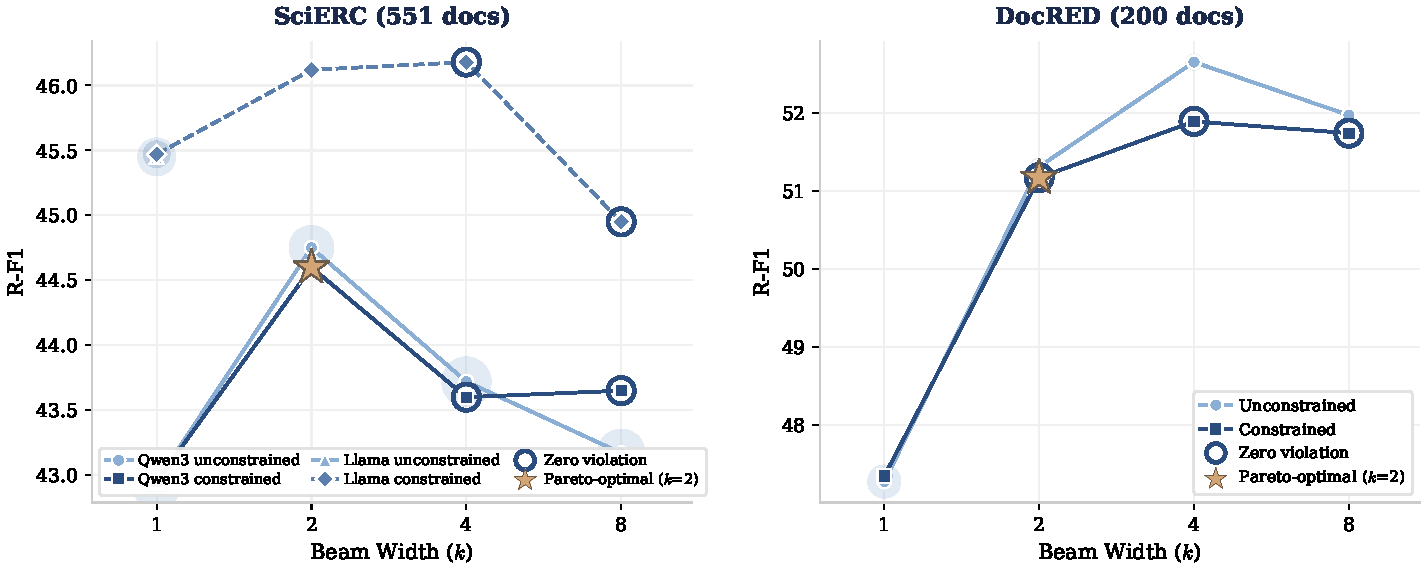
\includegraphics[width=\textwidth]{figures/beam_pareto.pdf}
\caption{Beam width vs.\ R-F1 under LoRA fine-tuning. Left: SciERC (Qwen3-8B solid, Llama-3.1-8B dashed; 551 docs). Right: DocRED (Llama-3.1-8B, 200 docs). Bubble area $\propto$ total violation rate (DR+CF+RV); rings mark zero-violation configurations. Star: Pareto-optimal ($k{=}2$).}
\label{fig:beam-pareto}
\end{figure*}

\begin{table}[h]
\centering
\small
\caption{Beam width sweep on SciERC (Qwen3-8B LoRA, 551 documents). \textsc{unc}: unconstrained; \textsc{con}: schema-constrained. Latency relative to $k{=}1$ unconstrained. Highlighted row: Pareto-optimal configuration.}
\label{tab:beam-sweep}
\resizebox{\columnwidth}{!}{%
\begin{tabular}{@{}cl cccc cc@{}}
\toprule
$k$ & Mode & E-F1 & R-F1 & DR (\%) & CF (\%) & Latency (s) & Rel.\ Lat. \\
\midrule
\multirow{2}{*}{1}
 & \textsc{unc} & 66.88 & 42.95 & 2.11 & 0    & 2.494 & 1.00$\times$ \\
 & \textsc{con} & 66.88 & 42.95 & \textbf{0} & 0.50 & 2.932 & 1.18$\times$ \\
\midrule
\multirow{2}{*}{2}
 & \textsc{unc} & 67.79 & 44.75 & 1.54 & 0    & 2.954 & 1.18$\times$ \\
 & \cellcolor{blue!8}\textsc{con} & \cellcolor{blue!8}67.71 & \cellcolor{blue!8}\textbf{44.60} & \cellcolor{blue!8}\textbf{0} & \cellcolor{blue!8}0.11 & \cellcolor{blue!8}3.463 & \cellcolor{blue!8}1.39$\times$ \\
\midrule
\multirow{2}{*}{4}
 & \textsc{unc} & 67.49 & 43.72 & 1.89 & 0    & 3.485 & 1.40$\times$ \\
 & \textsc{con} & 67.22 & 43.60 & \textbf{0} & 0    & 4.069 & 1.63$\times$ \\
\midrule
\multirow{2}{*}{8}
 & \textsc{unc} & 66.40 & 43.17 & 1.77 & 0    & 4.194 & 1.68$\times$ \\
 & \textsc{con} & 66.36 & 43.65 & \textbf{0} & 0    & 5.058 & 2.03$\times$ \\
\bottomrule
\end{tabular}}
\end{table}

\paragraph{Composability with fine-tuning.}
Under greedy decoding, the fine-tuned Qwen3-8B (LoRA, SciERC) with S1 constraints already achieves DR=0\% but retains CF=1.18\% (22 cross-field violations across 551 documents), with E-F1=67.05 and R-F1=43.77.
Adding beam search ($k{=}4$) eliminates all residual CF violations (1.18\%\,$\to$\,0\%), yielding zero violations across all four metrics (ET=0\%, RV=0\%, DR=0\%, CF=0\%) while preserving extraction quality (E-F1=66.88, R-F1=43.60; changes within $\pm$0.5\,pp).
Llama-3.1-8B (LoRA, SciERC) with S1 constraints and beam search ($k{=}4$) likewise achieves zero violations across all four metrics (ET=0\%, RV=0\%, DR=0\%, CF=0\%) with R-F1=46.18; the zero-violation result thus generalizes across calibrated model families.
The three constraint mechanisms (grammar masking, semantic domain-range filtering, and beam exploration) are thus fully composable: each addresses a distinct violation source without interfering with the others or degrading task performance.

The initial 50-document DocRED subset (Table~\ref{tab:beam-search}) was subsequently validated on the full 998-document set (Table~\ref{tab:beam-docred-998-zs}): both models achieve DR${=}$0\%, confirming subset representativeness.
Llama shows the larger improvement (CF 8.54\%\,$\to$\,1.00\%, 88\% reduction; R-F1 $+$2.6\,pp), consistent with beam search resolving constraint-search failures that greedy decoding cannot.

\begin{table}[h]
\centering
\small
\caption{Zero-shot beam search ($k{=}4$) under S1 constraints on the full DocRED dev set (998 documents).
ET/RV/DR/CF: violation rates (\%); PF: parse failure rate (\%); F1 $\times$100.}
\label{tab:beam-docred-998-zs}
\begin{tabular}{@{}lcccccc@{}}
\toprule
\textbf{Model} & ET & RV & DR$\,\downarrow$ & CF$\,\downarrow$ & E-F1$\,\uparrow$ & R-F1$\,\uparrow$ \\
\midrule
Qwen3-8B  & 0 & 0 & \textbf{0} & 4.94 & 58.19 & 8.72 \\
Llama-3.1-8B & 0 & 0 & \textbf{0} & 1.00 & 57.81 & 8.83 \\
\bottomrule
\end{tabular}
\end{table}

Table~\ref{tab:beam-docred-lora} reports LoRA + beam-4 results on the full DocRED dev set (998 documents), extending the fine-tuning composability evaluation from SciERC to the higher-$\bar{\kappa}$ regime.
Parse failure rates under LoRA beam-4 range from 1.3\% to 2.9\%, lower than the zero-shot rate.

\begin{table}[h]
\centering
\small
\caption{LoRA greedy vs.\ beam search ($k{=}4$) on DocRED (998 dev documents) under S1 constraints.
DR = domain/range, CF = cross-field violation rates (\%); PF = parse failure rate (\%); F1 $\times$ 100. ET and RV are 0\% in all rows.}
\label{tab:beam-docred-lora}
\resizebox{\columnwidth}{!}{%
\begin{tabular}{@{}llccccc@{}}
\toprule
\textbf{Model} & \textbf{Decoding} & DR$\,\downarrow$ & CF$\,\downarrow$ & E-F1$\,\uparrow$ & R-F1$\,\uparrow$ & PF \\
\midrule
\multirow{2}{*}{Qwen3-8B}
  & Greedy  & 0.01 & 0.41 & 81.43 & 40.56 & 8.52 \\
  & Beam-4  & \textbf{0} & 0.01 & 84.00 & 44.46 & 2.9 \\
\midrule
\multirow{2}{*}{Llama-3.1-8B}
  & Greedy  & 0.21 & 0.21 & 83.94 & 43.78 & 2.51 \\
  & Beam-4  & 0 & \textbf{0} & \textbf{85.23} & \textbf{47.17} & \textbf{1.3} \\
\bottomrule
\end{tabular}}
\end{table}

Llama-3.1-8B achieves zero violations across all four metrics (ET, RV, DR, CF = 0\%) on DocRED with LoRA + beam-4, extending the zero-violation result from SciERC to the high-$\bar{\kappa}$ regime.
Qwen3-8B achieves DR=0\% with near-zero CF (0.01\%); R-F1 is preserved ($\pm$0.06\,pp).
Combined with the sampling robustness results (Appendix~\ref{app:sampling}), these findings confirm that OntoCoDec's constraint enforcement is compatible with greedy, sampling, and beam search decoding without modification to the core constraint logic.

\paragraph{Latency overhead.}
Table~\ref{tab:beam-latency} reports wall-clock latency for greedy and beam search ($k{=}4$) under LoRA fine-tuning.

\begin{table}[h]
\centering
\small
\begin{tabular}{@{}lrr@{}}
\toprule
\textbf{Condition} & \textbf{s/doc} & \textbf{Overhead} \\
\midrule
Greedy unconstrained   & 2.612 & 1.00$\times$ \\
Greedy constrained (S1)& 2.873 & 1.10$\times$ \\
Beam-4 unconstrained   & 3.446 & 1.32$\times$ \\
Beam-4 constrained (S1)& 4.013 & 1.54$\times$ \\
\bottomrule
\end{tabular}
\caption{Latency per document (SciERC, 551 docs, Qwen3-8B LoRA FT, RTX PRO 6000 Blackwell). Overhead relative to greedy unconstrained.}
\label{tab:beam-latency}
\end{table}

Beam search itself adds 32\% latency (4 beams); constraint overhead increases from 10\% (greedy) to 17\% (beam) because each beam independently maintains grammar and semantic state.
Per-beam entity registry memory is $O(|\text{entities}|)$ per beam; at $k{=}8$ with typical document sizes, overhead is ${<}$1\,MB per beam, negligible relative to model memory.
The total 1.54$\times$ overhead is acceptable for offline batch IE; \texttt{early\_stopping} limits additional compute to partial-sequence exploration.

We also explored a type-consensus constraint that forces identical entity types across all relations within a document.
However, CF violations occur precisely where the consensus type conflicts with domain-range constraints, creating a fundamental CF$\leftrightarrow$DR trade-off.
With DR-aware enforcement (skipping consensus when it would violate domain-range), the layer becomes a no-op (100\% skip rate on 551 SciERC documents and 50 DocRED documents).
This confirms that beam search resolves the CF$\leftrightarrow$DR tension through a fundamentally different mechanism: token-level exploration of paths satisfying both constraints simultaneously.

\paragraph{TCR reranking under beam search.}
TCR reranking with beam search ($k{=}4$) showed no effect on either Qwen3-8B or Llama-3.1-8B under LoRA (0/551 SciERC candidates changed): fine-tuned beam candidates are already type-consistent (TCR score${=}$1.0 for all candidates), confirming that beam search implicitly subsumes post-hoc type consensus under fine-tuning.
This further strengthens the beam search deployment recommendation: beam achieves near-zero violations across all four types and renders post-hoc CF resolution unnecessary.
